\chapter{MIDI Setup}
\section{Connectivity}
\textbf{Machinedrum}
\begin{itemize}
    \item Connect the MIDI-Out of the Machinedrum to the MIDI-In (1) of the MegaCommand.
    \item Connect the MIDI-Out (1) of the MegaCommand to MIDI-In of the Machinedrum.
\end{itemize}

\textbf{Elektron Device (Analog4/MNM) (Optional)}
\begin{itemize}
    \item Connect the MIDI-Out of the Elektron to the MIDI-In (2) of the MegaCommand. 
    \item Connect the MIDI-Out (2) of the MegaCommand to MIDI-In of the Elektron.
\end{itemize}
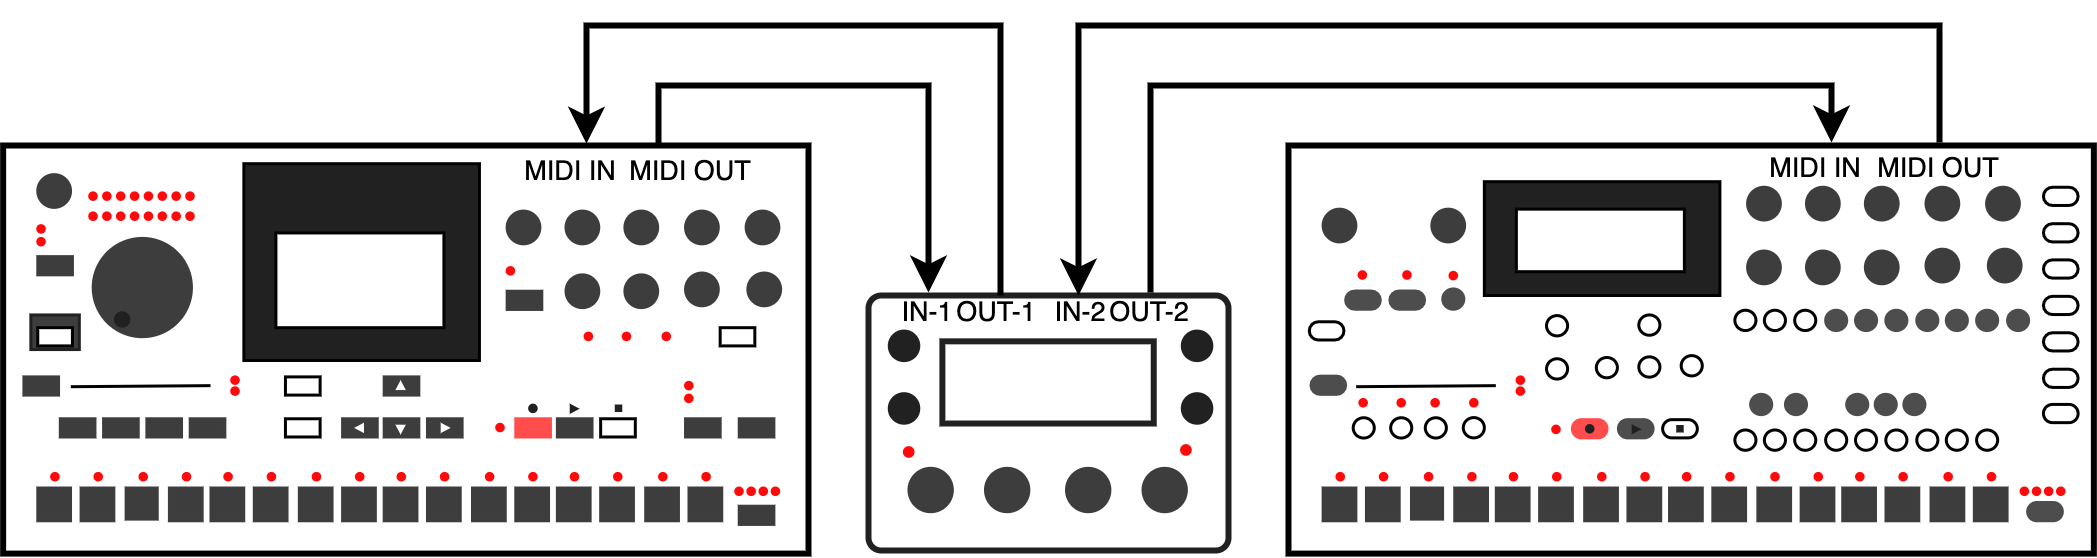
\includegraphics[width=16.55cm]{midi_machines.png}\\
\\
\textbf{External Clock (Optional)} 

\begin{itemize}
    \item A MIDI Keyboard, or sequencer can be connected to MIDI-In (2) , or USB MIDI. 
    \item Attached sequencers can be used as external clock source.
\end{itemize}

\textbf{External MIDI (Optional)}

\begin{itemize}
    \item A MIDI Keyboard connected to MIDI-In (2). 
    \item MIDI-Out (2) connected to synth a module's MIDI-In.
    \item Attached MIDI Keyboards may be used to play notes in chromatic modes or via the PianoRoll editor.
    \item External synth can be sequenced from the External Sequencer Tracks.
\end{itemize}



\newpage

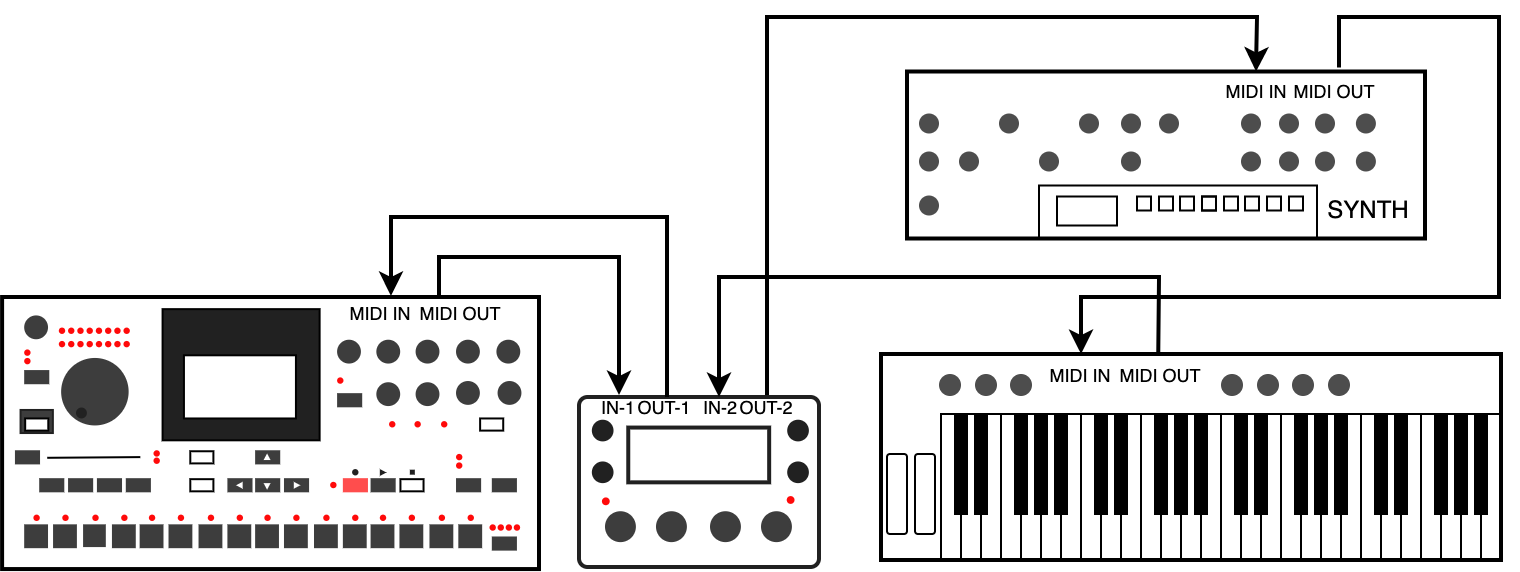
\includegraphics[width=18cm]{midi_machines2.png}\\
\section{MachineDrum Settings}
Upgrade your MD to the latest MDX OS.\\\\
MCL communicates with the MachineDrum using SYSEX messages, and will configure your MD's current global settings automatically.
\\\\The Machinedrum's base channel can be chosen from the MD's Global menu.\\\\
\textit{For MK1 models, Turbo Speed should be set no higher than 4x.\\(See Configuration Menu -> MIDI -> Port Config)}
\section{MonoMachine Settings}
Upgrade your MNM to the latest MNMX OS.\\\\
MCL communicates with the MonoMachine using SYSEX messages, and will configure your MNM's current global settings automatically.
\section{AnalogFour Settings}

The following configuration must be manually applied in the Analog 4's Global Settings menu:

\begin{itemize}

\item{MIDI Port Config:}
\begin{enumerate}
\item{Output to MIDI}
\item{Input to MIDI}
\item{Keyboard CFG = EXT}
\item{Receive Notes = True}
\item{Receive CC/NPRN = True}
\end{enumerate}
\item{MIDI Channels:}

Tracks 1-6 channels need to be set to MIDI Channels 1-6 respectively.

\end{itemize}
